\begin{ex}
 (Unesp-adaptado) Um jogo consiste num dispositivo eletrônico na forma de um círculo dividido em 10 setores iguais numerados como mostra a figura:
 \begin{center}
    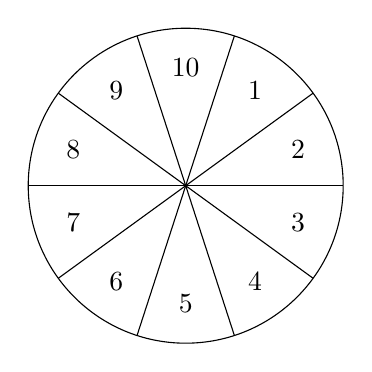
\begin{tikzpicture}
     \draw (0,0) circle [radius=2];
     \draw (0,0)--(2,0);
     \draw (0,0)--(1.618033989,1.175570505);
     \draw (0,0)--(0.6180339887,1.902113033);
     \draw (0,0)--(-0.6180339887,1.902113033);
     \draw (0,0)--(-1.618033989,1.175570505);
     \draw (0,0)--(-2,0);
     \draw (0,0)--(-1.618033989,-1.175570505);
     \draw (0,0)--(-0.6180339887,-1.902113033);
     \draw (0,0)--(0.6180339887,-1.902113033);
     \draw (0,0)--(1.618033989,-1.175570505);
     \draw (0,0)--(2,0);
     
     \node [] at (1.426584774,0.4635254916) {2};
     \node [] at (0.8816778784, 1.213525492) {1};
     \node [] at (0, 1.5) {10};
     \node [] at (-0.8816778784, 1.213525492) {9};
     \node [] at (-1.426584774,	0.4635254916) {8};
     \node [] at (-1.426584774,	-0.4635254916) {7};
     \node [] at (-0.8816778784, -1.213525492) {6};
     \node [] at (0,-1.5) {5};
     \node [] at (0.8816778784,-1.213525492) {4};
     \node [] at (1.426584774, -0.4635254916) {3};
     
    \end{tikzpicture}
 \end{center}
Em cada jogada, um único setor do círculo se ilumina. Todos os setores com números pares tem a mesma probabilidade de ocorrer, o mesmo acontecendo com os setores  de números ímpares. Além disso, a probabilidade de ocorrer o número 3 é o dobro da probabilidade de ocorrer o número 4. A probabilidade de, numa jogada, ocorrer um número primo maior ou igual a 2 é:
    \begin{enumerate}[(a)]
    \item $\frac{3}{5}$
    \item $\frac{7}{15}$
    \item $\frac{4}{15}$
    \item $\frac{13}{15}$
    \item $\frac{1}{3}$
    \end{enumerate}
      \begin{sol}
      resposta: b  \\
       $p(2)=p(4)=p(6)=p(8)=p(10)=x$ ;  $p(1)=p(3)=p(5)=p(7)=p(9)=2x$ \\ \\
       $\frac{p(2)+p(3)+p(5)+p(7)}{15x}=\frac{x+2x+2x+2x}{15x}=\frac{7}{15}$
      \end{sol}
\end{ex}